\documentclass{beamer}
\usetheme{Madrid}
\usepackage{amsmath}
\usepackage{ragged2e}
\graphicspath{ {./images/} }

\title{Introduction to Decision Trees}
\author{by Talentsprint Pvt. Ltd.}
\centering
\date{August 2020}

\begin{document}
\maketitle
\begin{frame}{Content}
	\begin{itemize}
		\item Decision Trees
		\item Types of Decision Trees
		\item Attribute Selection Measures
		\item Pruning
		\item Advantages and Disadvantage of Decision trees
		\item Overfitting and Underfitting
	\end{itemize}
\end{frame}

\begin{frame}{Decision Trees}
\begin{flushleft}
	It is a supervised learning algorithm. Unlike other supervised learning algorithms, it can be used for solving both regression and classification problems.
\vspace{10pt}

Decision Tree model can be used to predict the target variable by learning simple decision rules inferred from prior data.\\
\vspace{10pt}
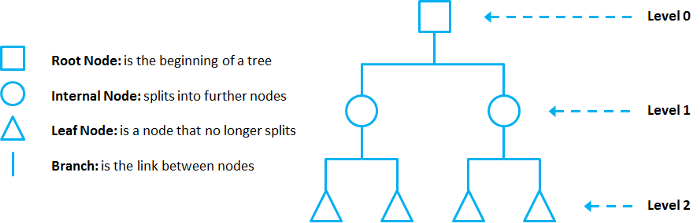
\includegraphics[scale=0.48]{DT_structure}
\end{flushleft}
\end{frame}

\begin{frame}{Types of Decision Trees}
	\begin{flushleft}
		Types of decision trees are based on the type of target variable we have. It can be of two types:

\begin{itemize}
	\item \textbf{Categorical Variable Decision Tree:} Decision Tree which has a categorical target variable then it called a Categorical variable decision tree.
	\item \textbf{Continuous Variable Decision Tree:} Decision Tree has a continuous target variable then it is called Continuous Variable Decision Tree.
\end{itemize}
\textbf{Types of DT Algorithms:}
\begin{itemize}
	\item ID3  - (Iterative Dichotomiser 3)
	\item C4.5 - (Successor of ID3)
	\item CART - (Classification And Regression Tree)
	\item CHAID- (Chi-square automatic interaction detection)
	\item MARS - (Multivariate Adaptive Regression Splines)
\end{itemize}
\end{flushleft}
\end{frame}

\begin{frame}{Attribute Selection Measures}
\begin{flushleft}
		\begin{itemize}
	\item \textbf{Entropy} : Measure of Impurity of Randomness
	\item \textbf{Information Gain} : Statistical property that measures how well a given attribute separates the training examples according to their target classification. 
	\item \textbf{Gini Index} : A cost function used to evaluate splits in the dataset
	\item \textbf{Gain Ratio} : Modification of IG for improved results
	\item \textbf{Reduction in Variance} : For Continuous target variable prediction using standard variance based splits.
	\item \textbf{Chi Square} : Statistical significance between the differences between sub-nodes and parent node. 
\end{itemize}
	\end{flushleft}
\end{frame}

\begin{frame}{Entropy}
\begin{flushleft}
		Entropy is a measure of the randomness in the information being processed. The higher the entropy, the harder it is to draw any conclusions from that information. Ex: Flipping a coin is an example of an action that provides information that is random.
\\
The Entropy is maximum when the probability is 0.5 because it projects perfect randomness in the data and there is no chance if perfectly determining the outcome.\\
\end{flushleft}

			$ E(S) = \sum_{i=1}^{c}{-p_i\log_2p_i} $
\begin{flushleft}
	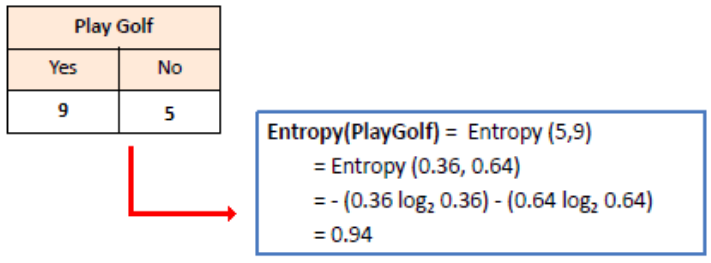
\includegraphics[scale=0.38]{Golf_example}
\end{flushleft}
\end{frame}

\begin{frame}{Information Gain}
\begin{flushleft}
		Information Gain is a measure of Entropy. The priority of features are identified using information gain. IG and priority are directly proportional to each other.
\end{flushleft}
	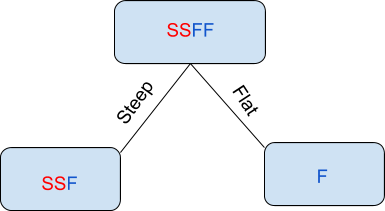
\includegraphics[scale=0.3]{Grade_split}
\begin{flushleft}
	 $ IG = E(parent)- (0.75*E(left node)+ 0.25*E(right node)) $ \\
	 $ IG = 1 - (0.75*0.91796214) + (0.25*0) $ \\
	 $ IG = 0.3112 $
\end{flushleft}
\end{frame}

\begin{frame}{Contd...}
\begin{flushleft}
	$ IG(Bumpiness) = E(parent) — (0.5 * E(bumpy) + 0.5 * E(smooth)) = 0 $ \\
	$ IG(Speed limit) = E(parent) — (0.5 * E(yes) + 0.5 * E(no)) = 1 $
	\end{flushleft}
	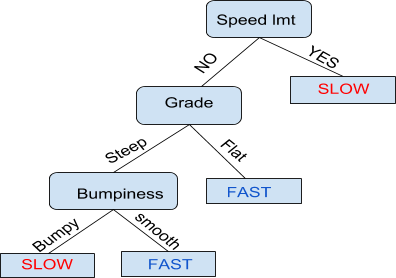
\includegraphics[scale=0.5]{DT_Car_example}
\end{frame}

\begin{frame}{Gini Index}
\begin{flushleft}
	 Gini index is a cost function used to evaluate splits in the dataset. It is calculated by subtracting the sum of the squared probabilities of each class from one. It favors larger partitions and easy to implement whereas information gain favors smaller partitions with distinct values.
		\begin{equation*}
			Gini = 1 - \sum_{i=1}^{c}(p_i)^2
		\end{equation*}
It works with the categorical target variable. It performs only Binary splits. Higher the value of Gini index higher the homogeneity.
\\
\vspace{10pt}
\textbf{Steps to Calculate Gini index for a split:}
\begin{itemize}
	\item Calculate Gini for sub-nodes, using the above formula for success(p) and failure(q) (p²+q²).
	\item Calculate the Gini index for split using the weighted Gini score of each node of that split.
\end{itemize}
CART uses the Gini index method to create split points.
	\end{flushleft}
\end{frame}

\begin{frame}{Gain Ratio}
\begin{flushleft}
	Information gain is biased towards choosing attributes with a large number of values as root nodes. It means it prefers the attribute with a large number of distinct values.

C4.5, an improvement of ID3, uses Gain ratio which is a modification of Information gain that reduces its bias and is usually the best option. Gain ratio overcomes the problem with information gain by taking into account the number of branches that would result before making the split. It corrects information gain by taking the intrinsic information of a split into account.
		\begin{equation*}
			Gain Ratio = \frac{IG}{SplitInfo} = \frac{Entropy(before)-\sum_{j=1}^{K}Entropy(j, after)}{\sum_{j=1}^{K}w_j\log_2w_j}
		\end{equation*}
Where “before” is the dataset before the split, K is the number of subsets generated by the split, and (j, after) is subset j after the split.

	\end{flushleft}
\end{frame}

\begin{frame}{Reduction in Variance}
\begin{flushleft}
	Reduction in variance is an algorithm used for continuous target variables (regression problems). This algorithm uses the standard formula of variance to choose the best split. The split with lower variance is selected as the criteria to split the population:
		\begin{equation*}
			Variance = \frac{\sum(X-\bar{X})^2}{n}
		\end{equation*}
X-bar is the mean of the values, X is actual and n is the number of values.

\textbf{Steps to calculate Variance:}
\begin{itemize}
	\item Calculate variance for each node.
	\item Calculate variance for each split as the weighted average of each node variance.
\end{itemize}

	\end{flushleft}
\end{frame}
\begin{frame}{Chi Square}
\begin{flushleft}
	It finds out the statistical significance between the differences between sub-nodes and parent node. We measure it by the sum of squares of standardized differences between observed and expected frequencies of the target variable.

It works with the categorical target variable “Success” or “Failure”. It can perform two or more splits. Higher the value of Chi-Square higher the statistical significance of differences between sub-node and Parent node.

It generates a tree called CHAID.
		\begin{equation*}
			\chi^2 = \sum\frac{(O-E)^2}{E}
		\end{equation*}
\textbf{Steps to calculate Chi-square for a split:}
\begin{itemize}
	\item Calculate Chi-square for an individual node by calculating the deviation for Success and Failure both.
	\item Calculated Chi-square of Split using Sum of all Chi-square of success and Failure of each node of the split.
\end{itemize}

	\end{flushleft}
\end{frame}
\begin{frame}{Pruning}
	\begin{flushleft}
	When a decision tree is built, many of the branches will reflect anomalies in the training data, due to noise or outliers. Slight changes in the values may result in completely different results.

Pruning the tree is one method that eradicates this by using statistical measures to remove the least reliable branches or the branches backed by a few number of samples.
\\
\vspace{10pt}
There are several approaches in Pruning:
\begin{itemize} 		
	\item \textbf{Pre-pruning} that stop growing the tree earlier, before it perfectly classifies the training set.
	\item \textbf{Post-pruning} that allows the tree to perfectly classify the training set, and then post prune the tree. 
\end{itemize}
Practically, the second approach of post-pruning overfit trees is more successful because it is not easy to precisely estimate when to stop growing the tree. 
	\end{flushleft}
\end{frame}
\begin{frame}{Advantages and Disadvantages of Decision Trees}
	\begin{flushleft}
		\textbf{Advantages:}
		\begin{itemize} 		
			\item Interpretable and Simple
			\item Handle all kinds of data
			\item Non-Parametric
			\item Robust
			\item Fast
		\end{itemize}
		\textbf{Disadvantages:}
		\begin{itemize} 		
			\item Overfitting
			\item Instability
			\item Bias
			\item Optimality
		\end{itemize}
	\end{flushleft}
\end{frame}
\begin{frame}{Overfitting and Underfitting}
	
\end{frame}
\begin{frame}
\huge{\centerline{The End}}
\end{frame}
\end{document}